\PassOptionsToPackage{unicode=true}{hyperref} % options for packages loaded elsewhere
\PassOptionsToPackage{hyphens}{url}
%
\documentclass[]{article}
\usepackage{lmodern}
\usepackage{amssymb,amsmath}
\usepackage{ifxetex,ifluatex}
\usepackage{fixltx2e} % provides \textsubscript
\ifnum 0\ifxetex 1\fi\ifluatex 1\fi=0 % if pdftex
  \usepackage[T1]{fontenc}
  \usepackage[utf8]{inputenc}
  \usepackage{textcomp} % provides euro and other symbols
\else % if luatex or xelatex
  \usepackage{unicode-math}
  \defaultfontfeatures{Ligatures=TeX,Scale=MatchLowercase}
\fi
% use upquote if available, for straight quotes in verbatim environments
\IfFileExists{upquote.sty}{\usepackage{upquote}}{}
% use microtype if available
\IfFileExists{microtype.sty}{%
\usepackage[]{microtype}
\UseMicrotypeSet[protrusion]{basicmath} % disable protrusion for tt fonts
}{}
\IfFileExists{parskip.sty}{%
\usepackage{parskip}
}{% else
\setlength{\parindent}{0pt}
\setlength{\parskip}{6pt plus 2pt minus 1pt}
}
\usepackage{hyperref}
\hypersetup{
            pdftitle={Logistic Regression - Answers},
            pdfauthor={SDS 291},
            pdfborder={0 0 0},
            breaklinks=true}
\urlstyle{same}  % don't use monospace font for urls
\usepackage[margin=1in]{geometry}
\usepackage{color}
\usepackage{fancyvrb}
\newcommand{\VerbBar}{|}
\newcommand{\VERB}{\Verb[commandchars=\\\{\}]}
\DefineVerbatimEnvironment{Highlighting}{Verbatim}{commandchars=\\\{\}}
% Add ',fontsize=\small' for more characters per line
\usepackage{framed}
\definecolor{shadecolor}{RGB}{248,248,248}
\newenvironment{Shaded}{\begin{snugshade}}{\end{snugshade}}
\newcommand{\AlertTok}[1]{\textcolor[rgb]{0.94,0.16,0.16}{#1}}
\newcommand{\AnnotationTok}[1]{\textcolor[rgb]{0.56,0.35,0.01}{\textbf{\textit{#1}}}}
\newcommand{\AttributeTok}[1]{\textcolor[rgb]{0.77,0.63,0.00}{#1}}
\newcommand{\BaseNTok}[1]{\textcolor[rgb]{0.00,0.00,0.81}{#1}}
\newcommand{\BuiltInTok}[1]{#1}
\newcommand{\CharTok}[1]{\textcolor[rgb]{0.31,0.60,0.02}{#1}}
\newcommand{\CommentTok}[1]{\textcolor[rgb]{0.56,0.35,0.01}{\textit{#1}}}
\newcommand{\CommentVarTok}[1]{\textcolor[rgb]{0.56,0.35,0.01}{\textbf{\textit{#1}}}}
\newcommand{\ConstantTok}[1]{\textcolor[rgb]{0.00,0.00,0.00}{#1}}
\newcommand{\ControlFlowTok}[1]{\textcolor[rgb]{0.13,0.29,0.53}{\textbf{#1}}}
\newcommand{\DataTypeTok}[1]{\textcolor[rgb]{0.13,0.29,0.53}{#1}}
\newcommand{\DecValTok}[1]{\textcolor[rgb]{0.00,0.00,0.81}{#1}}
\newcommand{\DocumentationTok}[1]{\textcolor[rgb]{0.56,0.35,0.01}{\textbf{\textit{#1}}}}
\newcommand{\ErrorTok}[1]{\textcolor[rgb]{0.64,0.00,0.00}{\textbf{#1}}}
\newcommand{\ExtensionTok}[1]{#1}
\newcommand{\FloatTok}[1]{\textcolor[rgb]{0.00,0.00,0.81}{#1}}
\newcommand{\FunctionTok}[1]{\textcolor[rgb]{0.00,0.00,0.00}{#1}}
\newcommand{\ImportTok}[1]{#1}
\newcommand{\InformationTok}[1]{\textcolor[rgb]{0.56,0.35,0.01}{\textbf{\textit{#1}}}}
\newcommand{\KeywordTok}[1]{\textcolor[rgb]{0.13,0.29,0.53}{\textbf{#1}}}
\newcommand{\NormalTok}[1]{#1}
\newcommand{\OperatorTok}[1]{\textcolor[rgb]{0.81,0.36,0.00}{\textbf{#1}}}
\newcommand{\OtherTok}[1]{\textcolor[rgb]{0.56,0.35,0.01}{#1}}
\newcommand{\PreprocessorTok}[1]{\textcolor[rgb]{0.56,0.35,0.01}{\textit{#1}}}
\newcommand{\RegionMarkerTok}[1]{#1}
\newcommand{\SpecialCharTok}[1]{\textcolor[rgb]{0.00,0.00,0.00}{#1}}
\newcommand{\SpecialStringTok}[1]{\textcolor[rgb]{0.31,0.60,0.02}{#1}}
\newcommand{\StringTok}[1]{\textcolor[rgb]{0.31,0.60,0.02}{#1}}
\newcommand{\VariableTok}[1]{\textcolor[rgb]{0.00,0.00,0.00}{#1}}
\newcommand{\VerbatimStringTok}[1]{\textcolor[rgb]{0.31,0.60,0.02}{#1}}
\newcommand{\WarningTok}[1]{\textcolor[rgb]{0.56,0.35,0.01}{\textbf{\textit{#1}}}}
\usepackage{longtable,booktabs}
% Fix footnotes in tables (requires footnote package)
\IfFileExists{footnote.sty}{\usepackage{footnote}\makesavenoteenv{longtable}}{}
\usepackage{graphicx,grffile}
\makeatletter
\def\maxwidth{\ifdim\Gin@nat@width>\linewidth\linewidth\else\Gin@nat@width\fi}
\def\maxheight{\ifdim\Gin@nat@height>\textheight\textheight\else\Gin@nat@height\fi}
\makeatother
% Scale images if necessary, so that they will not overflow the page
% margins by default, and it is still possible to overwrite the defaults
% using explicit options in \includegraphics[width, height, ...]{}
\setkeys{Gin}{width=\maxwidth,height=\maxheight,keepaspectratio}
\setlength{\emergencystretch}{3em}  % prevent overfull lines
\providecommand{\tightlist}{%
  \setlength{\itemsep}{0pt}\setlength{\parskip}{0pt}}
\setcounter{secnumdepth}{0}
% Redefines (sub)paragraphs to behave more like sections
\ifx\paragraph\undefined\else
\let\oldparagraph\paragraph
\renewcommand{\paragraph}[1]{\oldparagraph{#1}\mbox{}}
\fi
\ifx\subparagraph\undefined\else
\let\oldsubparagraph\subparagraph
\renewcommand{\subparagraph}[1]{\oldsubparagraph{#1}\mbox{}}
\fi

% set default figure placement to htbp
\makeatletter
\def\fps@figure{htbp}
\makeatother


\title{Logistic Regression - Answers}
\author{SDS 291}
\date{4/6/2020}

\begin{document}
\maketitle

{
\setcounter{tocdepth}{2}
\tableofcontents
}
We have data from each state (n=50) on their average income, education
(\% high school, \% college, and \% advanced degrees completed),
political leaning from a 2015 Gallup poll and whether President Trump
won that state (1=Win) or not (0=Did not Win) in the 2016 election.

\begin{verbatim}
## 'data.frame':    50 obs. of  8 variables:
##  $ State   : Factor w/ 50 levels "Alabama ","Alaska ",..: 1 2 3 4 5 6 7 8 9 10 ...
##  $ Abr     : Factor w/ 50 levels "AK","AL","AR",..: 2 1 4 3 5 6 7 8 9 10 ...
##  $ Income  : int  43623 72515 50255 41371 61818 60629 70331 60509 47507 49620 ...
##  $ HS      : num  84.3 92.1 86 84.8 81.8 90.7 89.9 88.4 86.9 85.4 ...
##  $ BA      : num  23.5 28 27.5 21.1 31.4 38.1 37.6 30 27.3 28.8 ...
##  $ Adv     : num  8.7 10.1 10.2 7.5 11.6 14 16.6 12.2 9.8 10.7 ...
##  $ Dem.Rep : int  -17 -17 -1 -7 16 -1 11 6 1 -4 ...
##  $ TrumpWin: int  1 1 1 1 0 0 0 0 1 1 ...
\end{verbatim}

\hypertarget{income-and-election-outcome}{%
\section{Income and Election
Outcome}\label{income-and-election-outcome}}

\hypertarget{plots}{%
\subsection{Plots}\label{plots}}

Below are two plots exploring the relationship between income and
President Trump winning that state. They are depicting the same pattern;
the second ``jitters'' the data.

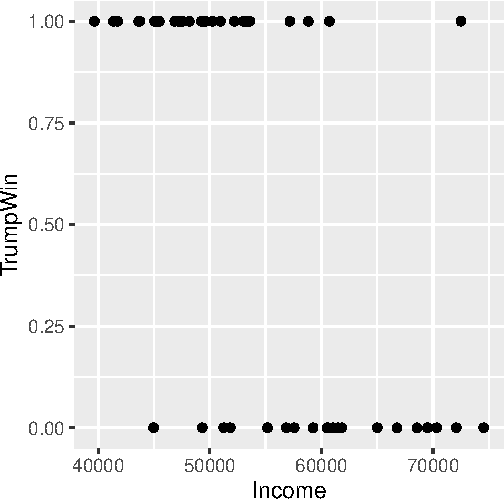
\includegraphics{17-class-exercise_answers_files/figure-latex/unnamed-chunk-2-1.pdf}
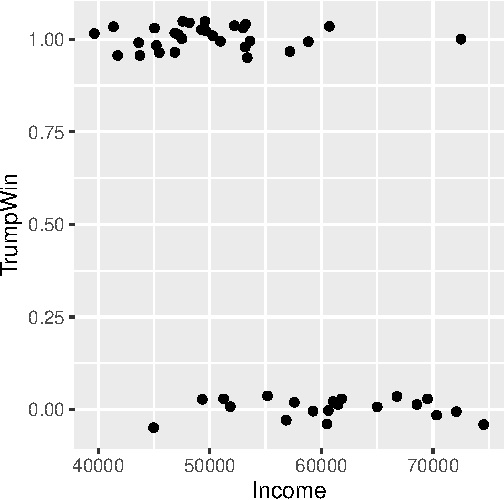
\includegraphics{17-class-exercise_answers_files/figure-latex/unnamed-chunk-2-2.pdf}

\begin{enumerate}
\def\labelenumi{\arabic{enumi}.}
\tightlist
\item
  Which is the easier graph to understand? Why?
\end{enumerate}

The right plot, with the jittered data makes the patterns more apparent
since the points aren't overlaying.

\begin{enumerate}
\def\labelenumi{\arabic{enumi}.}
\setcounter{enumi}{1}
\tightlist
\item
  What do you conclude from the plot about the relationship between
  income and the 2016 election results?
\end{enumerate}

The plot depicts a negative relationship between income and the 2016
election results. It is hard to determine the magnitude, but it seems
sort of moderately to weak, since there are a number of states with the
same average income that President Trump won and didn't win.

\hypertarget{logistic-model}{%
\subsection{Logistic Model}\label{logistic-model}}

Let's fit a logistic regression model to these data:
\(log(\frac{\pi}{1-\pi}) = \beta_0+\beta_1 X_1\)

Let's use Income in \$1,000s to make the interpretation a little easier.
Then we re-fit a logistic regression model.

\begin{Shaded}
\begin{Highlighting}[]
\NormalTok{Election16<-Election16 }\OperatorTok\StringTok{ }\KeywordTok{mutate}\NormalTok{(}\DataTypeTok{Income1000s =}\NormalTok{ Income}\OperatorTok{/}\DecValTok{1000}\NormalTok{)}
\NormalTok{m1<-}\KeywordTok{glm}\NormalTok{(TrumpWin}\OperatorTok{~}\NormalTok{Income1000s, }\DataTypeTok{data=}\NormalTok{Election16, }\DataTypeTok{family=}\NormalTok{binomial)}
\KeywordTok{summary}\NormalTok{(m1)}
\end{Highlighting}
\end{Shaded}

\begin{verbatim}
## 
## Call:
## glm(formula = TrumpWin ~ Income1000s, family = binomial, data = Election16)
## 
## Deviance Residuals: 
##     Min       1Q   Median       3Q      Max  
## -2.2049  -0.7510   0.4074   0.6566   2.5000  
## 
## Coefficients:
##             Estimate Std. Error z value Pr(>|z|)    
## (Intercept) 11.18186    3.07576   3.635 0.000277 ***
## Income1000s -0.19668    0.05582  -3.523 0.000426 ***
## ---
## Signif. codes:  0 '***' 0.001 '**' 0.01 '*' 0.05 '.' 0.1 ' ' 1
## 
## (Dispersion parameter for binomial family taken to be 1)
## 
##     Null deviance: 67.301  on 49  degrees of freedom
## Residual deviance: 45.923  on 48  degrees of freedom
## AIC: 49.923
## 
## Number of Fisher Scoring iterations: 5
\end{verbatim}

\begin{enumerate}
\def\labelenumi{\arabic{enumi}.}
\setcounter{enumi}{2}
\tightlist
\item
  Write the fitted regression model equation using the output above.
\end{enumerate}

\(log(odds) = 11.18186+-0.19668 Income1000s\)

\begin{enumerate}
\def\labelenumi{\arabic{enumi}.}
\setcounter{enumi}{3}
\tightlist
\item
  What is the direction and magnitude of the relationship between the
  average income and whether Pres.~Trump won that state?
\end{enumerate}

The association is negative and slight/shallow slope.

\begin{enumerate}
\def\labelenumi{\arabic{enumi}.}
\setcounter{enumi}{4}
\tightlist
\item
  Calculate the log(odds) (the book calls this the Empirical Logit), the
  odds, and the probability of President Trump winning for each of the
  following income levels. As a reminder, you can calculate each from
  the same output.
\end{enumerate}

\emph{Log(odds):} \[log(odds) = \beta_0+\beta_1 X_1\] \emph{Odds:}
\[Odds = e^{\beta_0+\beta_1 X_1}\] \emph{Probability:}
\[\pi = \frac{odds}{1+odds} = \frac{e^{\beta_0+\beta_1 X_1}}{1+e^{\beta_0+\beta_1 X_1}}\]

\begin{Shaded}
\begin{Highlighting}[]
\NormalTok{Income1000s<-}\KeywordTok{c}\NormalTok{(}\DecValTok{40}\OperatorTok{:}\DecValTok{70}\NormalTok{)}
\NormalTok{logodds<-}\KeywordTok{coef}\NormalTok{(m1)[}\DecValTok{1}\NormalTok{]}\OperatorTok{+}\StringTok{ }\NormalTok{(}\KeywordTok{coef}\NormalTok{(m1)[}\DecValTok{2}\NormalTok{]}\OperatorTok{*}\NormalTok{Income1000s)}
\NormalTok{m1_data<-}\KeywordTok{as.data.frame}\NormalTok{(}\KeywordTok{cbind}\NormalTok{(Income1000s,logodds))}
\NormalTok{m1_data <-}\StringTok{ }\NormalTok{m1_data }\OperatorTok
\StringTok{  }\KeywordTok{mutate}\NormalTok{(}\DataTypeTok{odds=}\KeywordTok{exp}\NormalTok{(logodds),}
        \DataTypeTok{prob =}\NormalTok{ odds}\OperatorTok{/}\NormalTok{(}\DecValTok{1}\OperatorTok{+}\NormalTok{odds))}
\end{Highlighting}
\end{Shaded}

\begin{longtable}[]{@{}llllllll@{}}
\toprule
Income & \$40,000 & \$50,000 & \$51,000 & \$55,000 & \$60,000 & \$61,000
& \$70,000\tabularnewline
\midrule
\endhead
Log(odds) & 3.315 & 1.348 & 1.151 & 0.365 & -0.619 & -0.815 &
-2.586\tabularnewline
Odds & 27.516 & 3.85 & 3.162 & 1.44 & 0.539 & 0.442 &
0.075\tabularnewline
Probability & 0.965 & 0.794 & 0.76 & 0.59 & 0.35 & 0.307 &
0.07\tabularnewline
\bottomrule
\end{longtable}

\begin{enumerate}
\def\labelenumi{\arabic{enumi}.}
\setcounter{enumi}{5}
\tightlist
\item
  Plot the values on each of the three plots below.
\end{enumerate}

Log(odds)

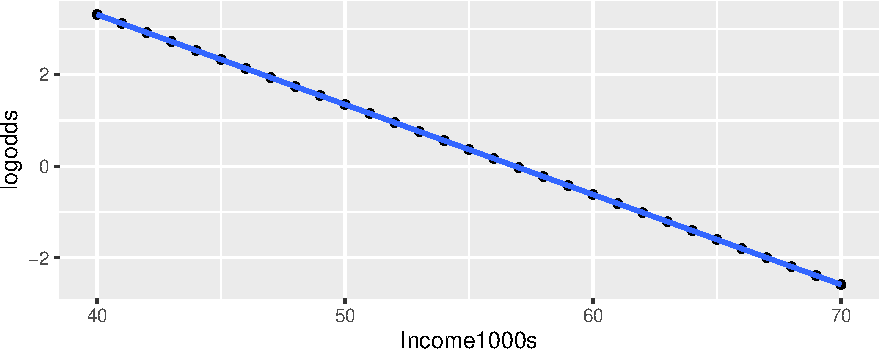
\includegraphics{17-class-exercise_answers_files/figure-latex/unnamed-chunk-5-1.pdf}

Odds

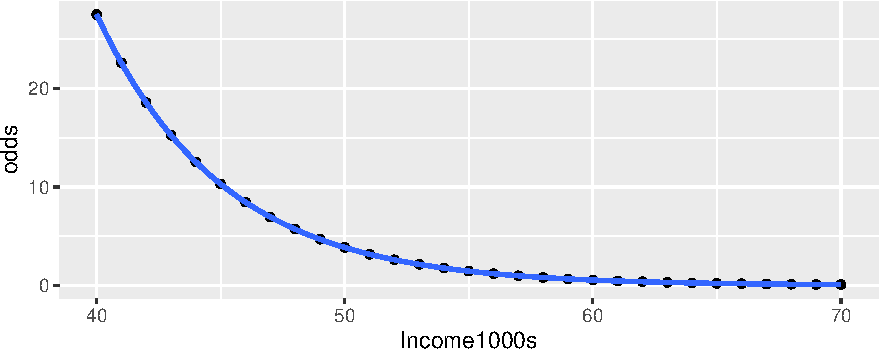
\includegraphics{17-class-exercise_answers_files/figure-latex/unnamed-chunk-6-1.pdf}

Probability

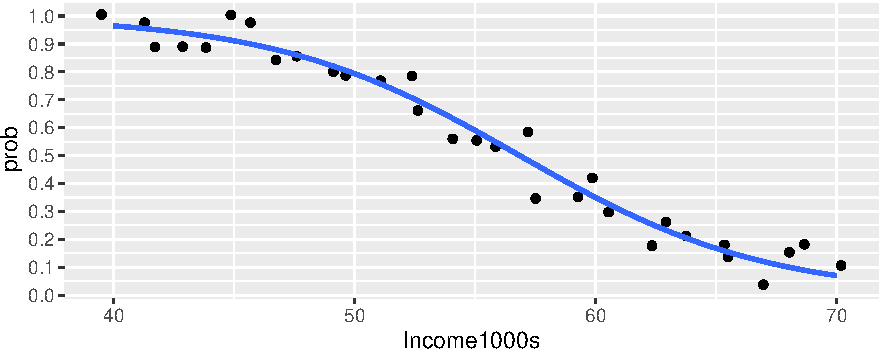
\includegraphics{17-class-exercise_answers_files/figure-latex/unnamed-chunk-7-1.pdf}

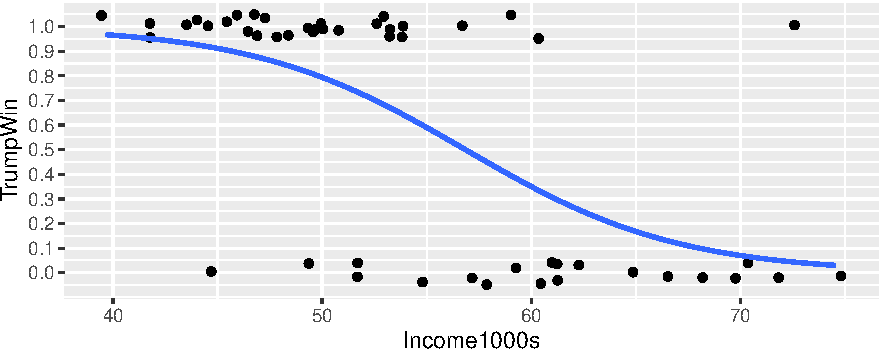
\includegraphics{17-class-exercise_answers_files/figure-latex/unnamed-chunk-8-1.pdf}

\begin{enumerate}
\def\labelenumi{\arabic{enumi}.}
\setcounter{enumi}{6}
\tightlist
\item
  What is the ratio of odds for President Trump winning a state?
\end{enumerate}

7a. Calculate the ratio the odds of a (theoretical) state with \$51,000
average income to a state with \$50,000 average income.

\begin{Shaded}
\begin{Highlighting}[]
\NormalTok{Odds51<-}\FloatTok{3.1623911}
\NormalTok{Odds50<-}\FloatTok{3.8497399}
\NormalTok{OR5051<-Odds51}\OperatorTok{/}\NormalTok{Odds50}
\NormalTok{OR5051}
\end{Highlighting}
\end{Shaded}

\begin{verbatim}
## [1] 0.8214558
\end{verbatim}

7b. Calculate the ratio the odds of a (theoretical) state with \$61,000
average income to a state with \$60,000 average income.

\begin{Shaded}
\begin{Highlighting}[]
\NormalTok{Odds61<-}\FloatTok{0.4424431}
\NormalTok{Odds60<-}\FloatTok{0.5386085}
\NormalTok{OR6061<-Odds61}\OperatorTok{/}\NormalTok{Odds60}
\NormalTok{OR6061}
\end{Highlighting}
\end{Shaded}

\begin{verbatim}
## [1] 0.8214558
\end{verbatim}

7c. Calculate the OR from the model (\(OR = e^{\beta_1}\)). Interpret
the odds ratio in a sentence.

\begin{Shaded}
\begin{Highlighting}[]
\KeywordTok{exp}\NormalTok{(}\KeywordTok{coef}\NormalTok{(m1)[}\DecValTok{2}\NormalTok{])}
\end{Highlighting}
\end{Shaded}

\begin{verbatim}
## Income1000s 
##   0.8214558
\end{verbatim}

Each additional \$1,000 average income was associated with 0.82 times
the odds of Trump winning in a state. States with \$1,000 higher average
income had a lower odds of Trump winning than a state with \$1,000 lower
average income.

7d. Did you get the same values from each approach? Why or why not?

Yes. Since we fit the logistic regression model as a linear model on the
log(odds) scale, the slope of the line, or the Odds Ratio, is constant,
just as a slope was in linear regression.

\begin{enumerate}
\def\labelenumi{\arabic{enumi}.}
\setcounter{enumi}{7}
\tightlist
\item
  Specify your hypotheses and conduct a test of whether the relationship
  between average income and President Trump winning a state is
  statistically signficant at the \(\alpha = 0.05\) level.
\end{enumerate}

\(H_0: \beta_1 = 0\)

\(H_0: \beta_1 \ne 0\)

We reject the null hypothesis since the test statistic for the
relationship between income and Trump winning was below the critical
value (-3.523\textless{}-1.96) and the associated p-value is below the
0.05 threshold (p\textless{}0.001).

\begin{enumerate}
\def\labelenumi{\arabic{enumi}.}
\setcounter{enumi}{8}
\tightlist
\item
  Calculate the 95\% Confidence Interval for the odds ratio of each
  additional \$1,000 of average income and of Pres Trump winning that
  state. \(t^* = 1.96\)
\end{enumerate}

\begin{Shaded}
\begin{Highlighting}[]
\NormalTok{lci<-}\KeywordTok{exp}\NormalTok{(}\OperatorTok{-}\FloatTok{0.19668} \OperatorTok{-}\StringTok{ }\NormalTok{(}\FloatTok{1.96}\OperatorTok{*}\FloatTok{0.05582}\NormalTok{))}
\NormalTok{uci<-}\KeywordTok{exp}\NormalTok{(}\OperatorTok{-}\FloatTok{0.19668} \OperatorTok{+}\StringTok{ }\NormalTok{(}\FloatTok{1.96}\OperatorTok{*}\FloatTok{0.05582}\NormalTok{))}
\NormalTok{CIs<-}\KeywordTok{cbind}\NormalTok{(lci,uci)}
\NormalTok{CIs}
\end{Highlighting}
\end{Shaded}

\begin{verbatim}
##            lci       uci
## [1,] 0.7363224 0.9164271
\end{verbatim}

Or get \texttt{R} to do it for you:

\begin{Shaded}
\begin{Highlighting}[]
\KeywordTok{exp}\NormalTok{(}\KeywordTok{confint}\NormalTok{(m1))}
\end{Highlighting}
\end{Shaded}

\begin{verbatim}
##                   2.5 %       97.5 %
## (Intercept) 366.9418556 7.917787e+07
## Income1000s   0.7232693 9.037885e-01
\end{verbatim}

\begin{enumerate}
\def\labelenumi{\arabic{enumi}.}
\setcounter{enumi}{9}
\tightlist
\item
  Create a binary variable of whether that state had above or below the
  national average rate of bachelor's degree holders (29.1\%) and repeat
  the steps above in \texttt{R}. (A note, these are the averages from
  these data, rather than from an external source that quoted a higher
  value. You might want to dichomoize at the median rather than the mean
  to avoid some very high/low BA degree states skewing the data, but
  nonethelesss, this is one approach.)
\end{enumerate}

\begin{Shaded}
\begin{Highlighting}[]
\NormalTok{Election16<-Election16 }\OperatorTok
\StringTok{  }\KeywordTok{mutate}\NormalTok{(}\DataTypeTok{Bach_Avg=}\KeywordTok{as.factor}\NormalTok{(}\KeywordTok{if_else}\NormalTok{(BA}\OperatorTok{>=}\DecValTok{29}\NormalTok{,}\StringTok{"Above"}\NormalTok{,}\StringTok{"Below"}\NormalTok{)))}
\NormalTok{Election16}\OperatorTok{$}\NormalTok{Bach_Avg <-}\StringTok{ }\KeywordTok{relevel}\NormalTok{(Election16}\OperatorTok{$}\NormalTok{Bach_Avg, }\DataTypeTok{ref=}\StringTok{"Below"}\NormalTok{)}

\NormalTok{Election16 }\OperatorTok
\StringTok{  }\KeywordTok{ggplot}\NormalTok{(}\KeywordTok{aes}\NormalTok{(}\DataTypeTok{y=}\NormalTok{TrumpWin, }\DataTypeTok{x=}\NormalTok{Bach_Avg)) }\OperatorTok{+}\StringTok{ }\KeywordTok{geom_jitter}\NormalTok{(}\DataTypeTok{width=}\FloatTok{0.1}\NormalTok{, }\DataTypeTok{height=}\FloatTok{0.05}\NormalTok{) }
\end{Highlighting}
\end{Shaded}

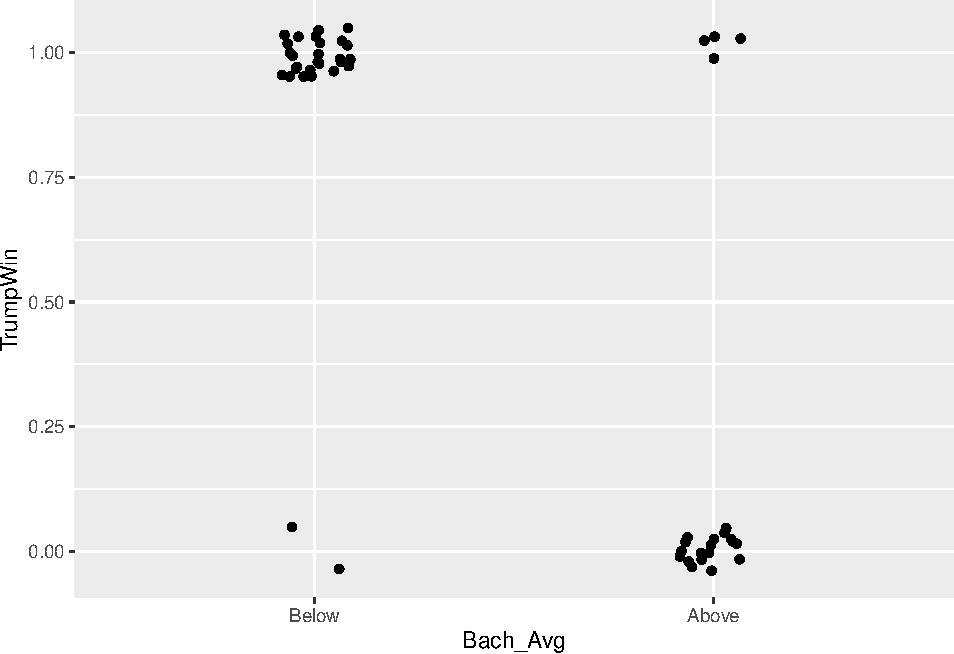
\includegraphics{17-class-exercise_answers_files/figure-latex/unnamed-chunk-14-1.pdf}

\begin{Shaded}
\begin{Highlighting}[]
\CommentTok{#another way to look at this is with a boxplot -- it will give you a solid line to indicate where most of the distribution is}
\NormalTok{Election16 }\OperatorTok
\StringTok{  }\KeywordTok{ggplot}\NormalTok{(}\KeywordTok{aes}\NormalTok{(}\DataTypeTok{y=}\NormalTok{TrumpWin, }\DataTypeTok{x=}\NormalTok{Bach_Avg)) }\OperatorTok{+}\StringTok{ }\KeywordTok{geom_boxplot}\NormalTok{()}
\end{Highlighting}
\end{Shaded}

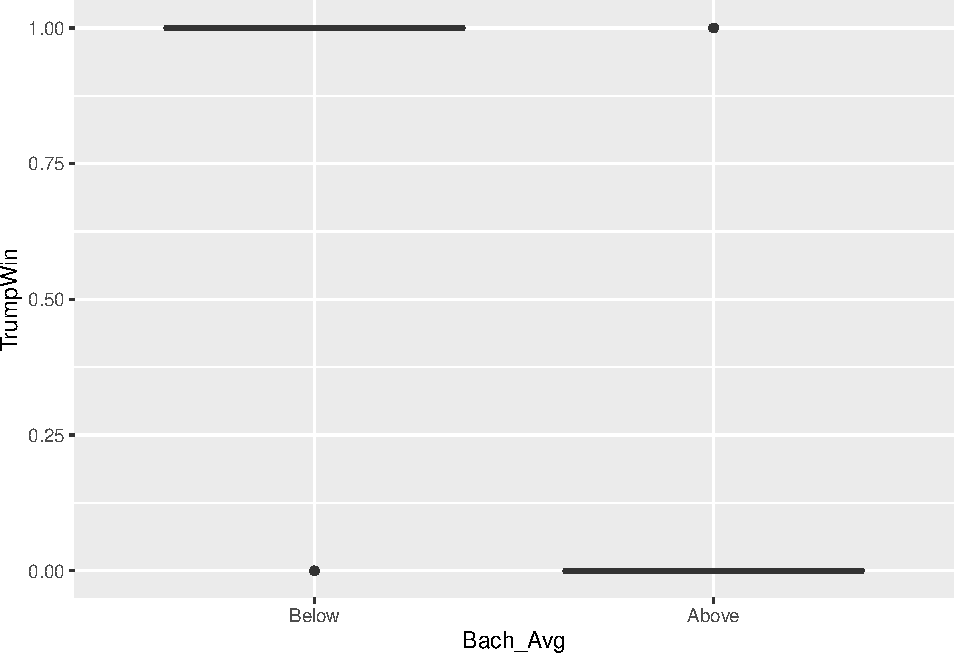
\includegraphics{17-class-exercise_answers_files/figure-latex/unnamed-chunk-14-2.pdf}

We see from the visual that being in a state that has higher than
average rates of bachelor's degree holders is negatively associated with
Trump winning those states.

\begin{Shaded}
\begin{Highlighting}[]
\KeywordTok{library}\NormalTok{(mosaic)}
\KeywordTok{tally}\NormalTok{(TrumpWin}\OperatorTok{~}\NormalTok{Bach_Avg, }\DataTypeTok{data=}\NormalTok{Election16)}
\end{Highlighting}
\end{Shaded}

\begin{verbatim}
##         Bach_Avg
## TrumpWin Below Above
##        0     2    18
##        1    26     4
\end{verbatim}

\begin{Shaded}
\begin{Highlighting}[]
\KeywordTok{tally}\NormalTok{(TrumpWin}\OperatorTok{~}\NormalTok{Bach_Avg, }\DataTypeTok{margins=}\OtherTok{TRUE}\NormalTok{, }\DataTypeTok{format =} \StringTok{"proportion"}\NormalTok{, }\DataTypeTok{data=}\NormalTok{Election16)}
\end{Highlighting}
\end{Shaded}

\begin{verbatim}
##         Bach_Avg
## TrumpWin      Below      Above
##    0     0.07142857 0.81818182
##    1     0.92857143 0.18181818
##    Total 1.00000000 1.00000000
\end{verbatim}

\begin{Shaded}
\begin{Highlighting}[]
\CommentTok{#}
\KeywordTok{library}\NormalTok{(gmodels)}
\KeywordTok{with}\NormalTok{(Election16, }\KeywordTok{CrossTable}\NormalTok{(TrumpWin, Bach_Avg,}
\DataTypeTok{prop.r=}\OtherTok{FALSE}\NormalTok{, }\DataTypeTok{prop.chisq=}\OtherTok{FALSE}\NormalTok{, }\DataTypeTok{prop.t=}\OtherTok{FALSE}\NormalTok{))}
\end{Highlighting}
\end{Shaded}

\begin{verbatim}
## 
##  
##    Cell Contents
## |-------------------------|
## |                       N |
## |           N / Col Total |
## |-------------------------|
## 
##  
## Total Observations in Table:  50 
## 
##  
##              | Bach_Avg 
##     TrumpWin |     Below |     Above | Row Total | 
## -------------|-----------|-----------|-----------|
##            0 |         2 |        18 |        20 | 
##              |     0.071 |     0.818 |           | 
## -------------|-----------|-----------|-----------|
##            1 |        26 |         4 |        30 | 
##              |     0.929 |     0.182 |           | 
## -------------|-----------|-----------|-----------|
## Column Total |        28 |        22 |        50 | 
##              |     0.560 |     0.440 |           | 
## -------------|-----------|-----------|-----------|
## 
## 
\end{verbatim}

\hypertarget{models}{%
\subsection{Models}\label{models}}

\begin{Shaded}
\begin{Highlighting}[]
\NormalTok{m2_}\DecValTok{2016}\NormalTok{<-}\KeywordTok{glm}\NormalTok{(TrumpWin}\OperatorTok{~}\NormalTok{Bach_Avg, }\DataTypeTok{data=}\NormalTok{Election16, }\DataTypeTok{family=}\NormalTok{binomial)}
\KeywordTok{summary}\NormalTok{(m2_}\DecValTok{2016}\NormalTok{)}
\end{Highlighting}
\end{Shaded}

\begin{verbatim}
## 
## Call:
## glm(formula = TrumpWin ~ Bach_Avg, family = binomial, data = Election16)
## 
## Deviance Residuals: 
##     Min       1Q   Median       3Q      Max  
## -2.2974  -0.6335   0.3850   0.3850   1.8465  
## 
## Coefficients:
##               Estimate Std. Error z value Pr(>|z|)    
## (Intercept)     2.5649     0.7338   3.495 0.000473 ***
## Bach_AvgAbove  -4.0690     0.9187  -4.429 9.46e-06 ***
## ---
## Signif. codes:  0 '***' 0.001 '**' 0.01 '*' 0.05 '.' 0.1 ' ' 1
## 
## (Dispersion parameter for binomial family taken to be 1)
## 
##     Null deviance: 67.301  on 49  degrees of freedom
## Residual deviance: 35.272  on 48  degrees of freedom
## AIC: 39.272
## 
## Number of Fisher Scoring iterations: 5
\end{verbatim}

\begin{Shaded}
\begin{Highlighting}[]
\CommentTok{#This code combines the odds ratios and the 95% CIs into three columns (OR, lower CI, Upper CI) for each of the terms in the model (here, just the intercept and the slope)}
\NormalTok{results_}\DecValTok{2016}\NormalTok{<-}\KeywordTok{exp}\NormalTok{(}\KeywordTok{cbind}\NormalTok{(}\KeywordTok{coef}\NormalTok{(m2_}\DecValTok{2016}\NormalTok{), }\KeywordTok{confint}\NormalTok{(m2_}\DecValTok{2016}\NormalTok{)))}
\end{Highlighting}
\end{Shaded}

\begin{verbatim}
## Waiting for profiling to be done...
\end{verbatim}

\begin{Shaded}
\begin{Highlighting}[]
\NormalTok{results_}\DecValTok{2016}
\end{Highlighting}
\end{Shaded}

\begin{verbatim}
##                                2.5 %      97.5 %
## (Intercept)   13.00000000 3.88861865 80.69732730
## Bach_AvgAbove  0.01709402 0.00208761  0.08559716
\end{verbatim}

A state with more than the national average of bachelor's degree holders
(i.e., a more highly educated state) has 0.017 times the odds of Trump
winning the state than a state with less than the national average of
bachelor degree holders. We are 95\% confident that the true
relationship between having above average amount of bachelor's degree
holders, compared to below average, and odds Trump winning is between
0.002 and 0.086. We can reject the null hypothesis (\(H_0: \beta_1 = 0\)
and \(H_A: \beta_1 \ne 0\)) and conclude that the association between a
state having an above average number of bachelor degree holders had
significantly lower odds of Trump winning than a state with below
average bachelor's degree holders, as evidenced by the large test
statstic (-4.429 \textless{} -1.96) and the small p-value (9.46e-06,
which is below our threshold of 0.05).

\hypertarget{recreating-the-above-with-the-elections-2008-data}{%
\section{Recreating the above with the Elections 2008
data}\label{recreating-the-above-with-the-elections-2008-data}}

The \texttt{Election16} data is in version 2.0 of the Stat2Data package,
which isn't yet on the server in the Stat2Data package. You could
practice with the \texttt{Election08} data, with the same variables
based on the 2008 election.

\begin{Shaded}
\begin{Highlighting}[]
\KeywordTok{data}\NormalTok{(}\StringTok{"Election08"}\NormalTok{)}
\NormalTok{Election08<-Election08 }\OperatorTok
\StringTok{  }\KeywordTok{mutate}\NormalTok{(}\DataTypeTok{Bach_Avg=}\KeywordTok{as.factor}\NormalTok{(}\KeywordTok{if_else}\NormalTok{(BA}\OperatorTok{>=}\FloatTok{27.14}\NormalTok{,}\StringTok{"Above"}\NormalTok{,}\StringTok{"Below"}\NormalTok{)),}
    \DataTypeTok{Income1000s =}\NormalTok{ Income}\OperatorTok{/}\DecValTok{1000}\NormalTok{)}
\NormalTok{Election08}\OperatorTok{$}\NormalTok{Bach_Avg <-}\StringTok{ }\KeywordTok{relevel}\NormalTok{(Election08}\OperatorTok{$}\NormalTok{Bach_Avg, }\DataTypeTok{ref=}\StringTok{"Below"}\NormalTok{)}
\end{Highlighting}
\end{Shaded}

\#Obama Winning and Income

\begin{Shaded}
\begin{Highlighting}[]
\NormalTok{Election08 }\OperatorTok
\StringTok{  }\KeywordTok{ggplot}\NormalTok{(}\KeywordTok{aes}\NormalTok{(}\DataTypeTok{y=}\NormalTok{ObamaWin, }\DataTypeTok{x=}\NormalTok{Income)) }\OperatorTok{+}\StringTok{ }\KeywordTok{geom_jitter}\NormalTok{(}\DataTypeTok{width =} \FloatTok{0.1}\NormalTok{, }\DataTypeTok{height=}\FloatTok{0.05}\NormalTok{)}
\end{Highlighting}
\end{Shaded}

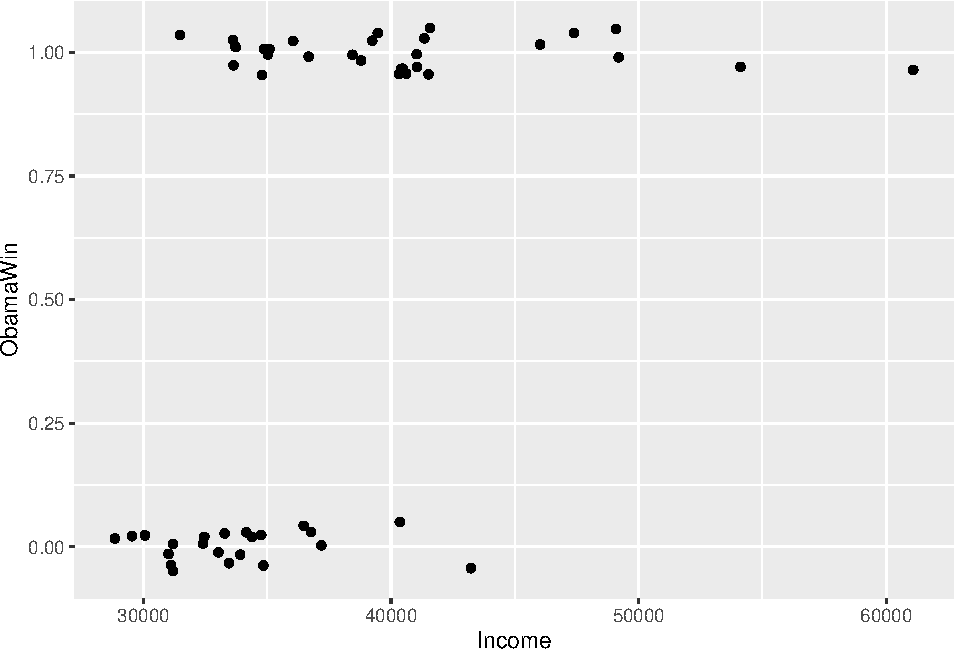
\includegraphics{17-class-exercise_answers_files/figure-latex/unnamed-chunk-18-1.pdf}

\begin{Shaded}
\begin{Highlighting}[]
\NormalTok{m1_}\DecValTok{2008}\NormalTok{<-}\KeywordTok{glm}\NormalTok{(ObamaWin}\OperatorTok{~}\NormalTok{Income1000s, }\DataTypeTok{data=}\NormalTok{Election08, }\DataTypeTok{family=}\NormalTok{binomial)}
\KeywordTok{summary}\NormalTok{(m1_}\DecValTok{2008}\NormalTok{)}
\end{Highlighting}
\end{Shaded}

\begin{verbatim}
## 
## Call:
## glm(formula = ObamaWin ~ Income1000s, family = binomial, data = Election08)
## 
## Deviance Residuals: 
##     Min       1Q   Median       3Q      Max  
## -2.3433  -0.7976   0.1329   0.6866   1.8124  
## 
## Coefficients:
##             Estimate Std. Error z value Pr(>|z|)    
## (Intercept) -12.4251     3.7522  -3.311 0.000928 ***
## Income1000s   0.3494     0.1050   3.328 0.000874 ***
## ---
## Signif. codes:  0 '***' 0.001 '**' 0.01 '*' 0.05 '.' 0.1 ' ' 1
## 
## (Dispersion parameter for binomial family taken to be 1)
## 
##     Null deviance: 69.737  on 50  degrees of freedom
## Residual deviance: 48.867  on 49  degrees of freedom
## AIC: 52.867
## 
## Number of Fisher Scoring iterations: 5
\end{verbatim}

\begin{Shaded}
\begin{Highlighting}[]
\CommentTok{#This code combines the odds ratios and the 95% CIs into three columns (OR, lower CI, Upper CI) for each of the terms in the model (here, just the intercept and the slope)}
\NormalTok{results1_}\DecValTok{2008}\NormalTok{<-}\KeywordTok{exp}\NormalTok{(}\KeywordTok{cbind}\NormalTok{(}\KeywordTok{coef}\NormalTok{(m1_}\DecValTok{2008}\NormalTok{), }\KeywordTok{confint}\NormalTok{(m1_}\DecValTok{2008}\NormalTok{)))}
\NormalTok{results1_}\DecValTok{2008}
\end{Highlighting}
\end{Shaded}

\begin{verbatim}
##                                 2.5 %      97.5 %
## (Intercept) 4.016472e-06 8.491176e-10 0.002563891
## Income1000s 1.418252e+00 1.185437e+00 1.799879223
\end{verbatim}

\#Obama Winning and Bachelor's Degrees

\begin{Shaded}
\begin{Highlighting}[]
\NormalTok{Election08 }\OperatorTok
\StringTok{  }\KeywordTok{ggplot}\NormalTok{(}\KeywordTok{aes}\NormalTok{(}\DataTypeTok{y=}\NormalTok{ObamaWin, }\DataTypeTok{x=}\NormalTok{Bach_Avg)) }\OperatorTok{+}\StringTok{ }\KeywordTok{geom_jitter}\NormalTok{(}\DataTypeTok{width =} \FloatTok{0.1}\NormalTok{, }\DataTypeTok{height=}\FloatTok{0.05}\NormalTok{)}
\end{Highlighting}
\end{Shaded}

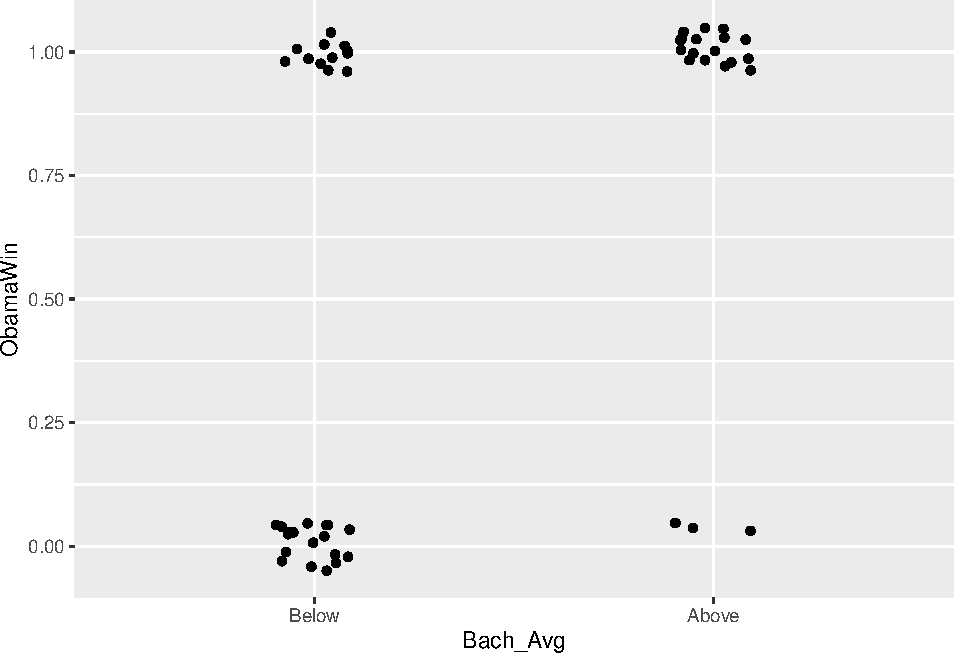
\includegraphics{17-class-exercise_answers_files/figure-latex/unnamed-chunk-19-1.pdf}

\begin{Shaded}
\begin{Highlighting}[]
\NormalTok{m2_}\DecValTok{2008}\NormalTok{<-}\KeywordTok{glm}\NormalTok{(ObamaWin}\OperatorTok{~}\NormalTok{Bach_Avg, }\DataTypeTok{data=}\NormalTok{Election08, }\DataTypeTok{family=}\NormalTok{binomial)}
\KeywordTok{summary}\NormalTok{(m2_}\DecValTok{2008}\NormalTok{)}
\end{Highlighting}
\end{Shaded}

\begin{verbatim}
## 
## Call:
## glm(formula = ObamaWin ~ Bach_Avg, family = binomial, data = Election08)
## 
## Deviance Residuals: 
##     Min       1Q   Median       3Q      Max  
## -1.9479  -0.9895   0.5701   0.5701   1.3777  
## 
## Coefficients:
##               Estimate Std. Error z value Pr(>|z|)   
## (Intercept)    -0.4595     0.3687  -1.246  0.21268   
## Bach_AvgAbove   2.1941     0.7267   3.019  0.00253 **
## ---
## Signif. codes:  0 '***' 0.001 '**' 0.01 '*' 0.05 '.' 0.1 ' ' 1
## 
## (Dispersion parameter for binomial family taken to be 1)
## 
##     Null deviance: 69.737  on 50  degrees of freedom
## Residual deviance: 58.289  on 49  degrees of freedom
## AIC: 62.289
## 
## Number of Fisher Scoring iterations: 4
\end{verbatim}

\begin{Shaded}
\begin{Highlighting}[]
\CommentTok{#This code combines the odds ratios and the 95% CIs into three columns (OR, lower CI, Upper CI) for each of the terms in the model (here, just the intercept and the slope)}
\NormalTok{results2_}\DecValTok{2008}\NormalTok{<-}\KeywordTok{exp}\NormalTok{(}\KeywordTok{cbind}\NormalTok{(}\KeywordTok{coef}\NormalTok{(m2_}\DecValTok{2008}\NormalTok{), }\KeywordTok{confint}\NormalTok{(m2_}\DecValTok{2008}\NormalTok{)))}
\NormalTok{results2_}\DecValTok{2008}
\end{Highlighting}
\end{Shaded}

\begin{verbatim}
##                             2.5 %    97.5 %
## (Intercept)   0.6315789 0.2981381  1.285685
## Bach_AvgAbove 8.9722222 2.3993648 44.638041
\end{verbatim}

\end{document}
